\documentclass[a4paper]{article}

\usepackage[english]{babel}
\usepackage[utf8]{inputenc}
\usepackage{amsmath}
\usepackage{graphicx}
\usepackage[colorinlistoftodos]{todonotes}
\usepackage{apacite}
\usepackage[round, sort, numbers, authoryear]{natbib}
\usepackage{hyperref}

\title{Bubble shooter}

\author{
    Bavdaz, Luka\\
    \texttt{4228561}
    \and
    Clark, Liam\\
    \texttt{4303423}
    \and
    Gmelig Meyling, Jan-Willem\\
    \texttt{4305167}
    \and
    Hoek, Leon\\
    \texttt{4021606}
    \and
    Smulders, Sam\\
    \texttt{4225007}
}

\date{\today}

\begin{document}
\maketitle

% \begin{abstract}
% Your abstract.
% \end{abstract}

\section{The Core}
\subsection{Responsibilities and collaborations of the main classes}
The first important class is the GUI class, which is responsible for the user interface, as all buttons are contained there. Furthermore, it contains one JPanels containing the the game objects. It has a run method that calls the gameStep method of the cannon every frame.

The cannon class is responsible for converting mouse input to actions the cannon can take and managing all the bubbles that come in contact with the cannon untill they collide with the bubbleMesh. It is also responsible for drawing the cannon.

Another important class is the bubbleMesh class that is responsible for all the logic regarding the popping of bubbles, adding new rows of bubbles and checking for game ending conditions. It contains all the non moving bubbles.

\subsection{Less important classes}
Other classes are less important because they contain mostly information about themselves instead of other objects. One missing responsibility is the lack of a class to manage all the game objects on the field. Also, the  cannon class has multiple responsibilities: managing the cannon, handeling user input and managing the bubble shot by the cannon. To repair this, a new class is introduced: The Room class.

Most central to the game logic is the Room class, which has the responsibility of containing all game objects of one player's side of the field. It is responsible for instantiating the game objects and calling their gameStep and render methods. Among other objects, it contains a cannon, the bubblequeue of bubbles that will be shot, the moving bubble that is shot and the bubbleMesh. The Room class takes the place of the cannon class as one of the main classes.

The cannon class is now only responsible for drawing the cannon and recieves its input from a newly added cannon controller using an observer, which is also a main class. An additional benefit of this architecture is the ability to change how the cannon is controlled without modifying the cannon class.

Other classes did not have similar or little responsibilities and were kept as they were before.

\subsection{class diagram of the main elements}
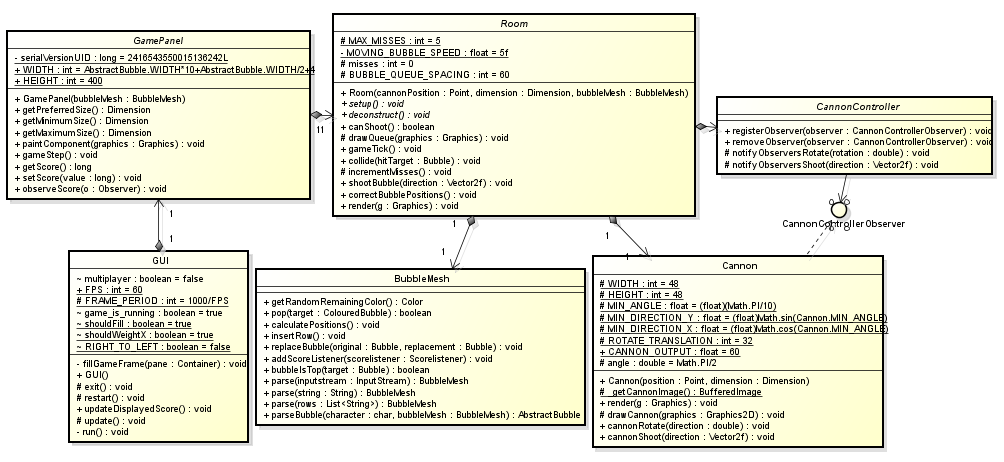
\includegraphics[width=1\textwidth]{main_classes_diagram_v2_picture.PNG}
%\caption{\label{fig:classesdiagram}These are the main classes of the project, along with the GamePanel class that connects the GUI to the Room.}

\subsection{sequence diagram of the main elements}
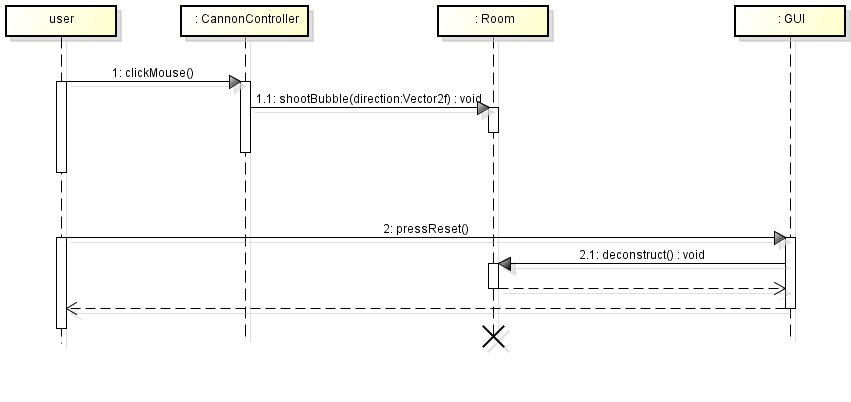
\includegraphics[width=1\textwidth]{AAAAA_plaatje.PNG}

\section{Theory in practice}
\subsection{Aggregation and composition}
Both terms refer to the relationship between a containing class and a member object. The difference lies in the possibility for the member object to exist without the owner. In aggregation, the member object can exist without the owner. In  composition, an object contains other objects that cannot exist without the owner.

Our project uses composition mostly, since the member objects generally cannot exist without the containing class. The cannon and the bubblemesh are always inside the same room; without the room these member objects cannot exist. Aggregation is used when the member object is a bubble. The bubbles are created within the room, where they are placed in the queue. They do not stay there, since they can be shot and absorbed into the bubblemesh, thus being able to exist without either containing class.

\subsection{Hierarchies}
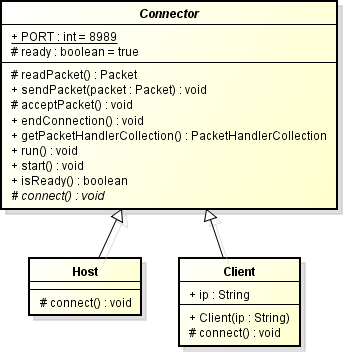
\includegraphics[width=1\textwidth]{Connector_Inher.png}
Figure 1

In figure 1, the Host and Client, share most of their responsibilities. So this is a case of the Host and Client is\_a Connector. Also the classes who use the Host and/or Client, treat the classes in the same way. Both classes are used for sending and accepting packets in the same way. So there is polymorphism involved.


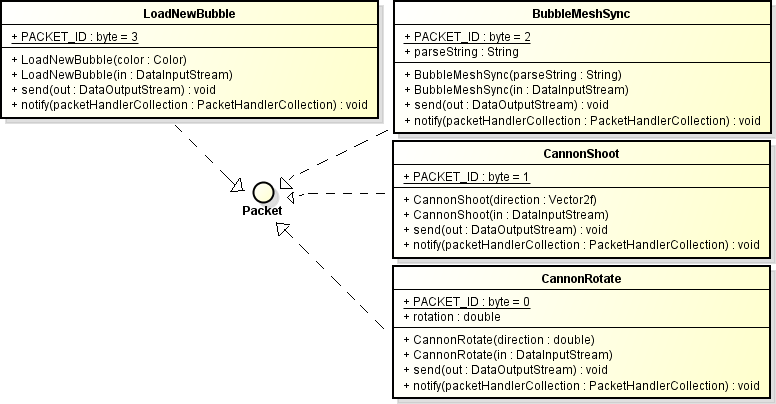
\includegraphics[width=1\textwidth]{PacketInher.png}
Figure2

In figure 2, we use polymorphism, because all packets share in how they are treated when they are being send.

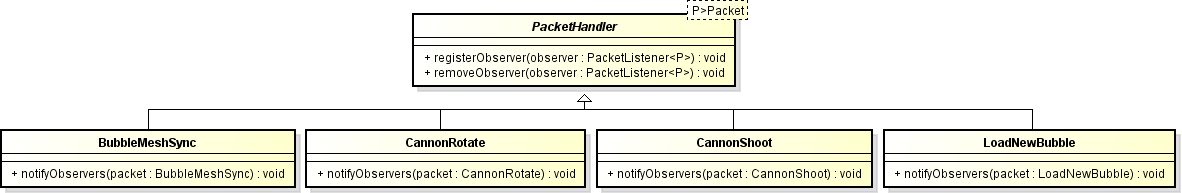
\includegraphics[width=1\textwidth]{PacketHandlerInher.png}
Figure3

The hierachy of figure 3 is a case of is\_a. All classes are PacketHandlers, they are all responsible for sending Packets to their observers.

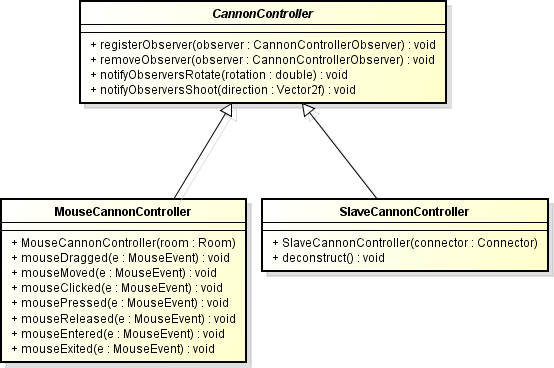
\includegraphics[width=1\textwidth]{CannonControllerInher.png}
Figure4

The reason for inheritance for the CannonController in figure 4 is both, polymorphism and is\_a. Both classes should determine the behaviour of the cannon and they should both be able to be observed in the same way, so they do share responsibilities. So for both classes is\_a CannonController. Also polymorphism is involved, both classes are uniformly treated as in the CannonController is determined.

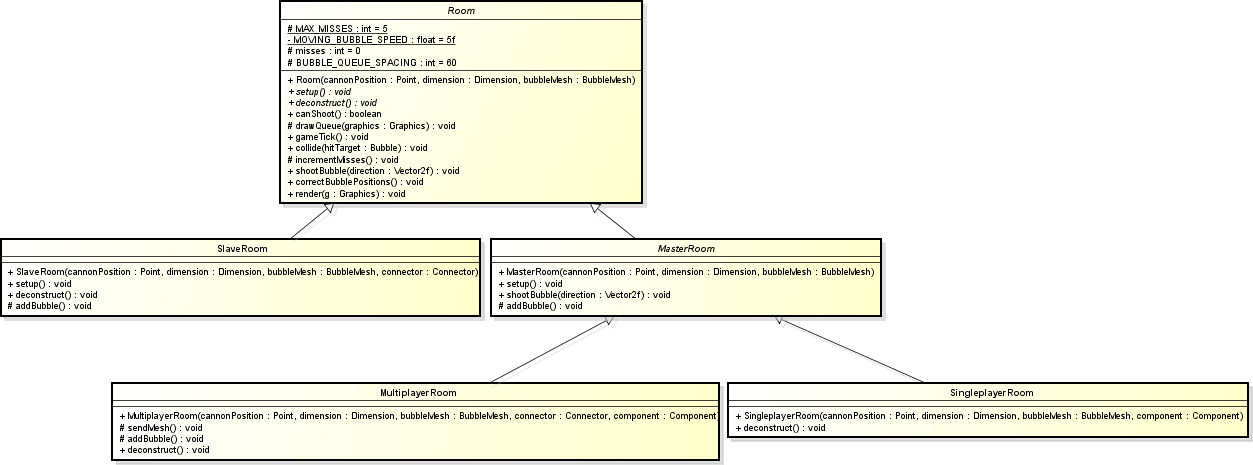
\includegraphics[width=1\textwidth]{RoomInher.png}
Figure 5

In the hierarchy in figure 5, there is a case of is\_a, all classes share responsibilities. Also polymorphism is involved, all classes are uniformly treated as in the Room is determined. We choose to add an extra layer between the MultiplayerRoom and SingleplayerRoom between Room, because both have in common that they determine themselves what happens in the room, while the SlaveRoom asks the Connector, by receiving Packets, to determine what to do.

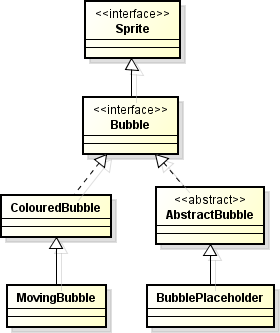
\includegraphics[width=1\textwidth]{bubbleInher.png}
Figure 6

In figure 6 we use both generalisation and realisation. On the top of the heirarchy, we got the Bubble interface extending the Sprite interface. The Bubble should behave like a Sprite, since every Bubble should be able to be drawn. So here we use polymorphism.
The ColouredBubble and AbstractBubble should both beheave like a Bubble, so here we use polymorphism again.
For the MovingBubble we use �is � a�, because the MovingBubble is a ColouredBubble with an extra behaviour.
For the BubblePlaceholder we use �is � a� and polymorphism, we use polymorphism because we expect to add more AbstractBubble classes, and we want to tread them in the same way as the AbstractBubble. �is � a� because BubblePlaceHolder shares responsibilities with AbstractBubble.



\subsection{Ifs and switches}
We placed a switch in the nl.tudelft.ti2206.network.packets.PacketFactory.class, the here switch is necessary to detect the difference between the raw data of packages before we can reconstruct the packages.

We left an if statement in nl.tudelft.ti2206.cannon.MouseCannonController.class, here we calculate the right angle for the cannon from raw data from the MouseMovementListener.

In the Room class, all if statements are used for null checking. This could be replaced by creating a 'null' class for each, class where we use a null-check on, but we decieded that this would overcomplicate our architecture.

In the Connector we use if statements to check if the inputstream, outputstream and socket are initialised, before we try to close them, since this might not be the case when the connection enstablishment fails.

In the GUI class if statements are used to check if the game is running in the multiplayer game mode. Using double dispatch instead of checking of a boolean flag would require adding classes with little or overlapping responsibilities.

To determine if a MovingBubble has left the playing field if statements are used. These cannot be removed because they evaluate inequalities required for the game logic.

In the AbstractBubble class, if statements are used to calculate a relative position to another bubble. For each direction, a special offset is added to the position of the neighbouring bubble. These offsets are the same for one type of direction (for example: top left), however, we haven't been able to change this if statement into a iterative statement (for each binding), because the current logic requires bindings to be checked in a given order to avoid infinte looping.

%we need to fix the bubbles!

\pagebreak


\end{document}
